\chapter{Introduction}

Population geneticist are historians telling the story of evolution. Mutation and recombination leave faithful historical records in the genome of every single organism on earth. The records have always been there, but over the past decades, the experimental and computational tools to decipher those records have improved dramatically. This introductory chapter surveys several key methodological trends that have transformed population genetic research, and finally delineates how these trends have built up the momentum for the original work presented in this thesis.

\section{Genealogical modeling of evolution using the \acl{ARG}}

%% Intro from pedigree to ARG, explain coalescence and recombination
The genetic relationships between ancestors and descendants form the basis of all evolutionary genomics research. The simplest data structure that encodes ancestor-descendant relationships is a pedigree, commonly known as a ``family tree". 

\begin{figure}%[h]
    \centering
    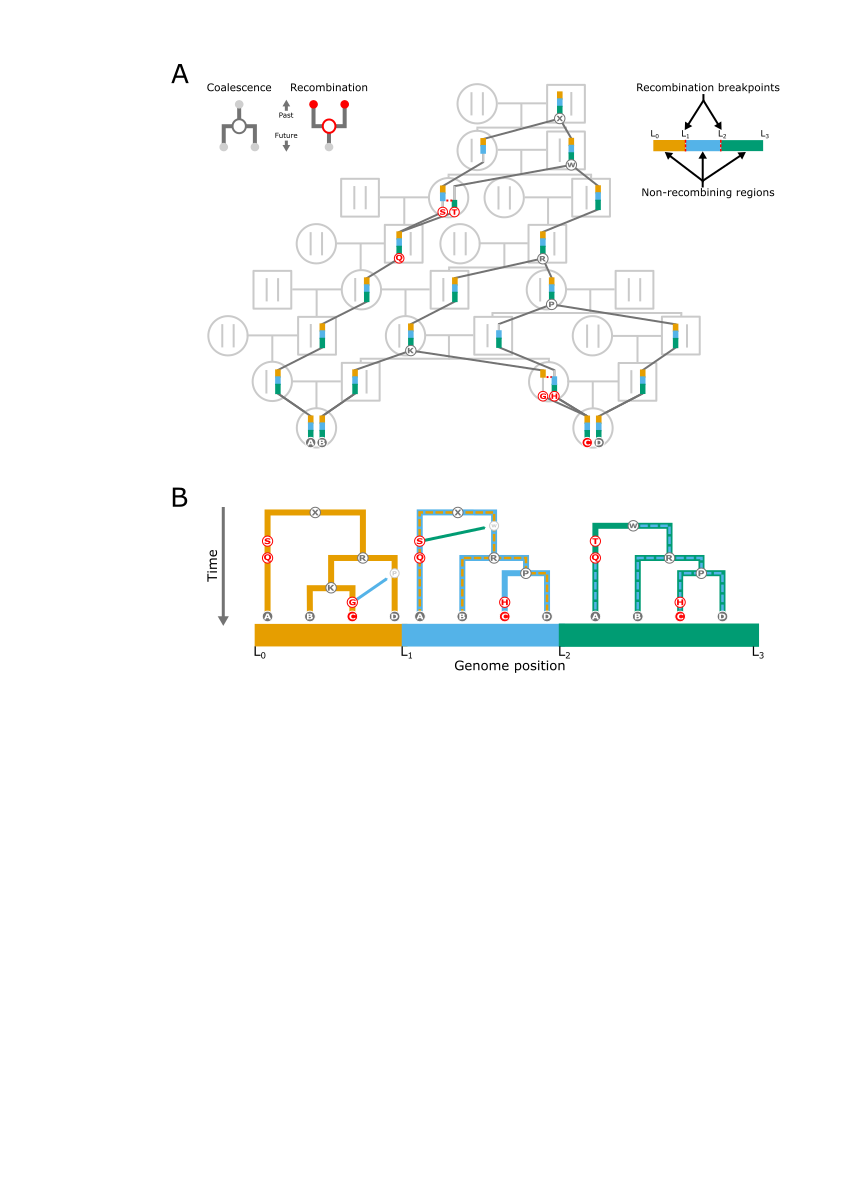
\includegraphics[width=\textwidth]{adapted_figs/arg_illustration.png}
    \caption[The \acf{ARG}]{\textbf{The \acf{ARG}}. Adapted from \cite{lewanski2023era} under a \href{https://creativecommons.org/licenses/by/4.0/}{CC BY 4.0} license.}
    \label{fig:intro-F1}
\end{figure}

% talk about tree representation

%% Utilities of ARGs

%% ARG inference methods

%% Existing work built on ARGs

%%% Fig. legend A) graphical representation of an ARG embedded in a pedigree B) tree-sequence representation

\section{Population-genetic simulations power large-scale \textit{in silico} experiments of evolution}

%% Types of simulations -> hybrid/ recapitation, accelerate

%% ARG simulations

%% The tree-sequence format and tskit

%% finally, catelog of simulations, stdpopsim, benchmark methods, empiricist easier

\section{\ac{AI}/\ac{ML} methods for biomedical sciences}

\section{Studies of selective sweeps generate key insights into adaptive evolution}

\section{Objectives and outline of thesis}
